\section{Spiral galaxy simulation}\label{sec:spiral-galaxy-sim}
The parameters used in the simulation of a spiral galaxy are shown in \autoref{tab:galaxy-parameters}.
\begin{table}[htp]
    \centering
    \caption{Galaxy model parameters used in the simulation.}
    \label{tab:galaxy-parameters}
    \begin{tabular}{lc}
        \toprule
        \textbf{Parameter}   & \textbf{Value}           \\
        \midrule
        Halo radius          & 3 kpc                    \\
        Halo mass            & $60 \times 10^9 M_\odot$ \\
        Disk radius          & 15 kpc                   \\
        Disk mass            & $15 \times 10^9 M_\odot$ \\
        Disk thickness       & 0.3 kpc                  \\
        Disk density profile & Uniformly decreasing     \\
        \bottomrule
    \end{tabular}
\end{table}
The galaxy is simulated as an isolated system; however, in deriving \autoref{eq:poisson-fourier-product}, periodic boundary conditions were assumed.
The simplest way (and the one used) to obtain a free-space solution from the PM method is to extend the computational domain twice in every dimension and fill the space unused in mass distribution with zeros.
The total size of the potential mesh used was $128 \times 128 \times 64$ with the region of interest occupying a box of size $60\, \text{kpc}\times 60\, \text{kpc}\times 30\, \text{kpc}$ located in a $64 \times 64 \times 32$ octant of the mesh.

\subsection{PM method}
In the PM method, $N=50{,}000$ particles were used.
Cell size $H$ and timestep length were set to $60/64=0.9375$ kpc and 1 Myr, respectively.
For convenience, the full configuration of the PM method is presented in \autoref{tab:pm-method-parameters}.
\begin{table}[htp]
    \centering
    \caption{PM method configuration.}
    \label{tab:pm-method-parameters}
    \begin{tabular}{lc}
        \toprule
        \textbf{Parameter}      & \textbf{Value}                     \\
        \midrule
        Effective mesh size     & $64 \times 64 \times 32$           \\
        $H$ (cell size)         & $60/64=0.9375$ kpc                 \\
        DT (time step)          & $1$ Myr                            \\
        Mass assignment scheme  & TSC                                \\
        Finite difference       & Two-point                          \\
        Green's function        & Derived from discretized Laplacian \\
        Time integration method & Leapfrog                           \\
        Number of particles     & 50,000                             \\
        \bottomrule
    \end{tabular}
\end{table}
The system's evolution over 200 Myr is shown in \autoref{fig:spiral-galaxy-evolution-pm}.

\begin{figure}[!ht]
    \centering
    \begin{subfigure}[b]{0.45\textwidth}
        \centering
        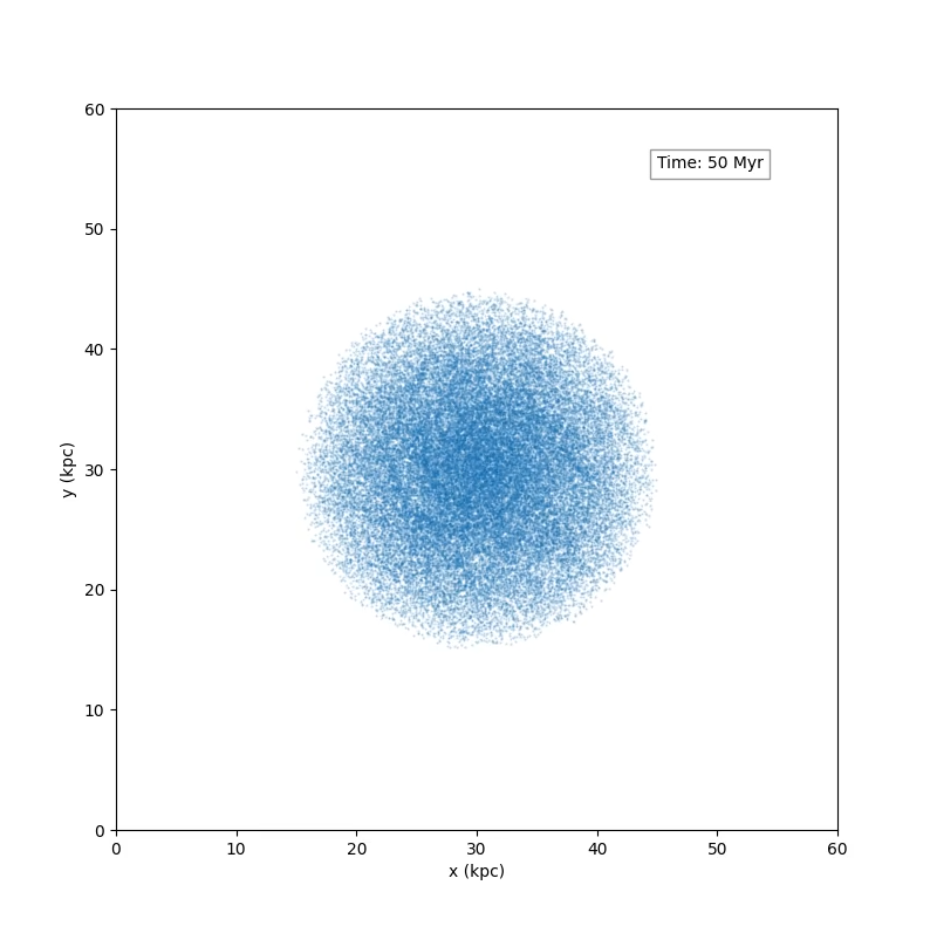
\includegraphics[width=\textwidth]{chapters/results/img/pm-galaxy/50myr.png}
        \caption{$t=50\,\text{Myr}$}
        \label{fig:spiral-galaxy-evolution-pm-sub1}
    \end{subfigure}
    \hfill
    \begin{subfigure}[b]{0.45\textwidth}
        \centering
        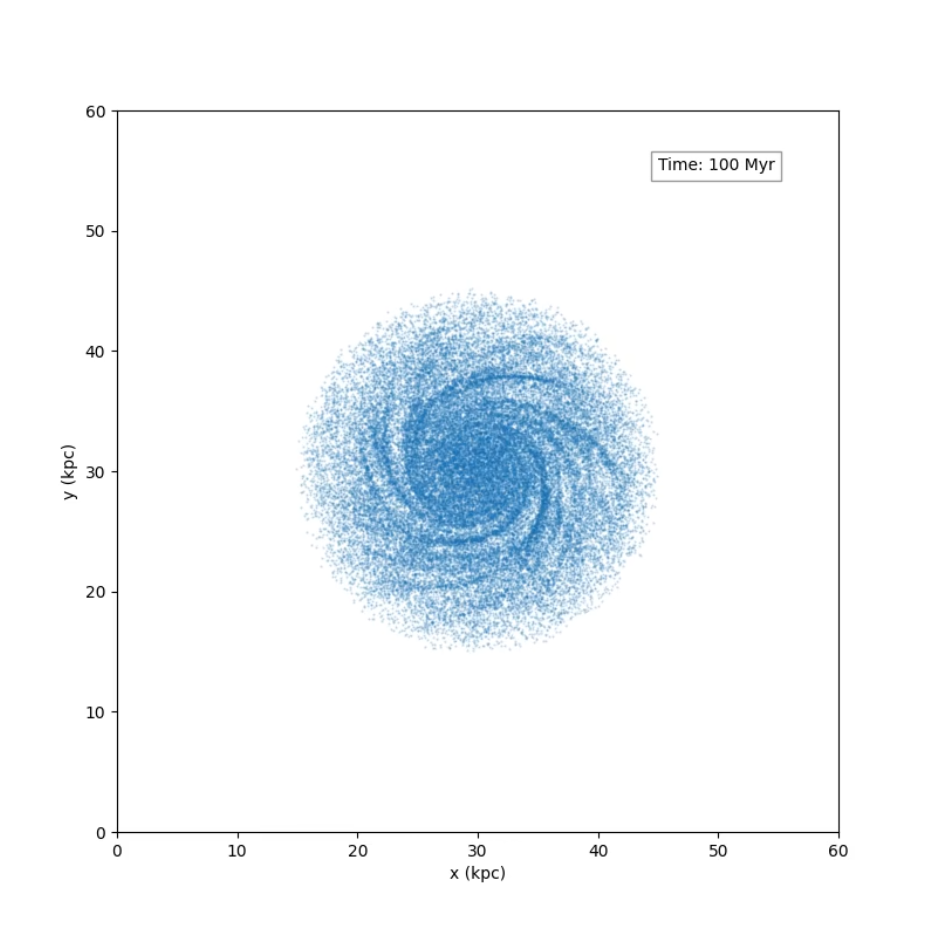
\includegraphics[width=\textwidth]{chapters/results/img/pm-galaxy/100myr.png}
        \caption{$t=100\,\text{Myr}$}
        \label{fig:spiral-galaxy-evolution-pm-sub2}
    \end{subfigure}

    \vspace{0.2cm}

    \begin{subfigure}[b]{0.45\textwidth}
        \centering
        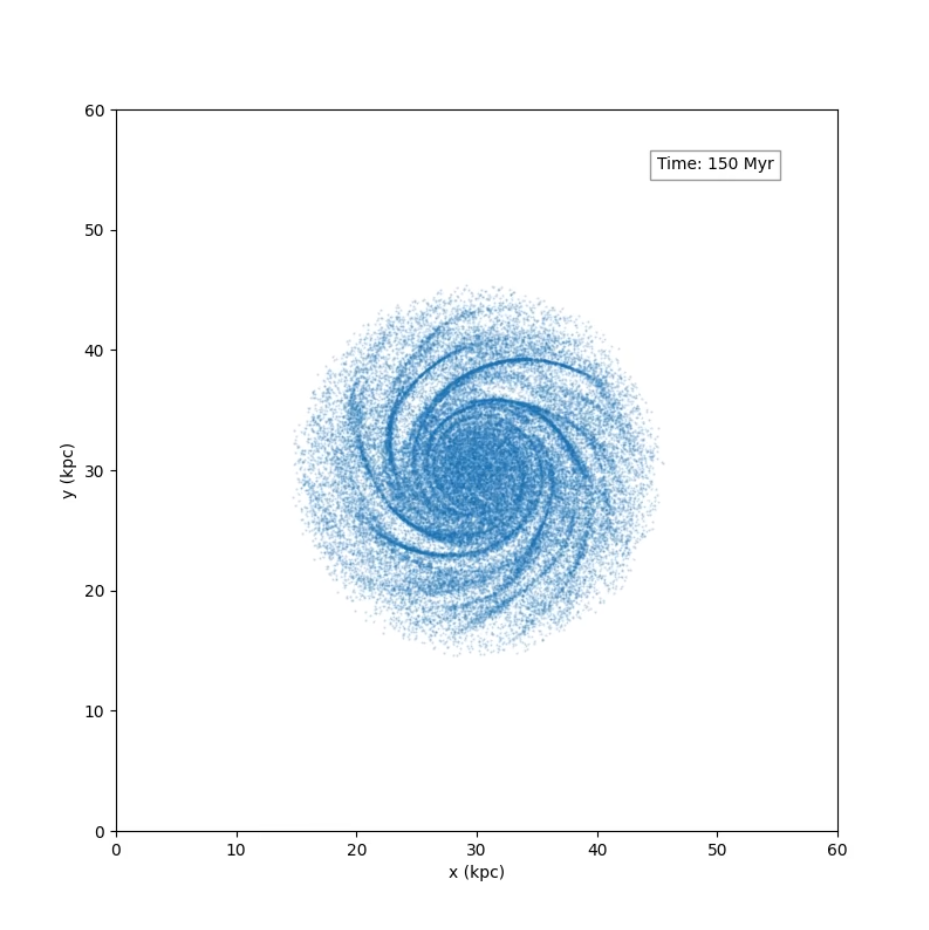
\includegraphics[width=\textwidth]{chapters/results/img/pm-galaxy/150myr.png}
        \caption{$t=150\,\text{Myr}$}
        \label{fig:spiral-galaxy-evolution-pm-sub3}
    \end{subfigure}
    \hfill
    \begin{subfigure}[b]{0.45\textwidth}
        \centering
        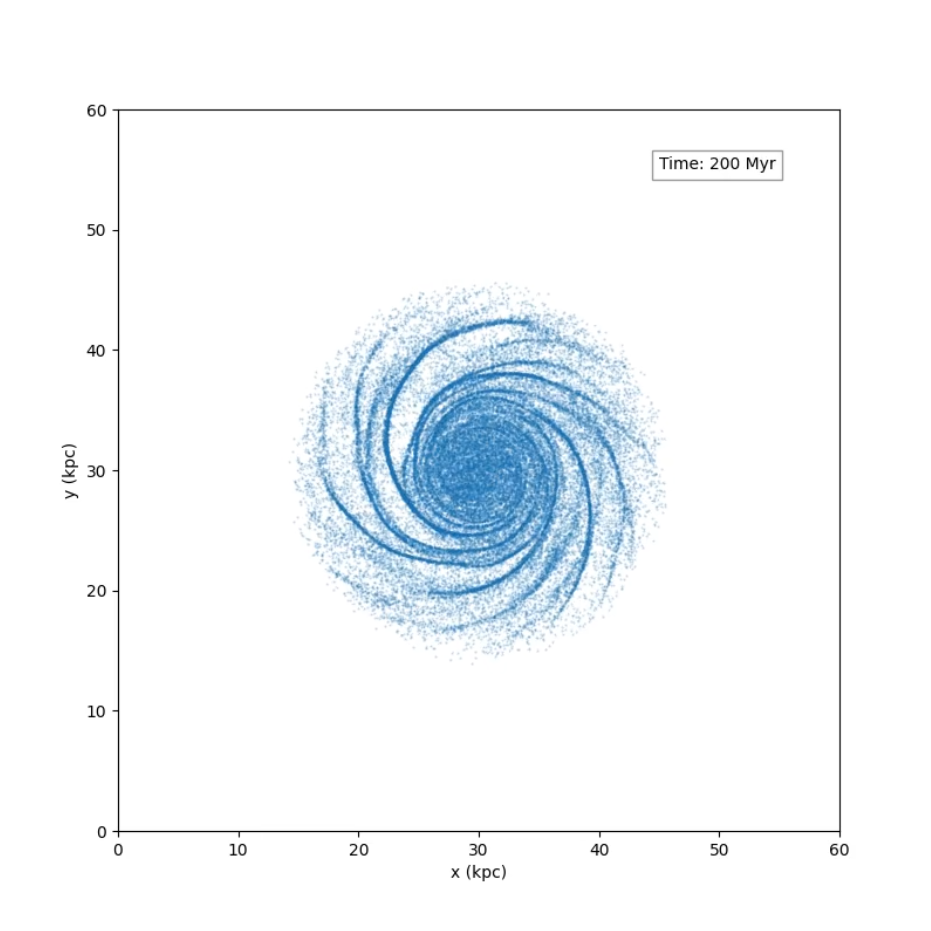
\includegraphics[width=\textwidth]{chapters/results/img/pm-galaxy/200myr.png}
        \caption{$t=200\,\text{Myr}$}
        \label{fig:spiral-galaxy-evolution-pm-sub4}
    \end{subfigure}

    \caption{Evolution of a spiral galaxy as predicted by the PM method.}
    \label{fig:spiral-galaxy-evolution-pm}
\end{figure}

During the simulation, total energy $E = \textrm{KE} + \textrm{PE}$, angular momentum $\mathbf{l}$, and the $z$-component of the momentum vector $\mathbf{p}$ should stay constant.
The $x$- and $y$-components of momentum change due to the presence of an external gravitational field (representing the halo) that exerts force $\mathbf{F}^\text{ext}$ on the system.
We can verify if this variation satisfies the expected relation
\begin{equation}\label{eq:expected-momentum-change}
    \dot{\mathbf{p}} = \mathbf{F}^\text{ext}
\end{equation}
by finding the initial total momentum $\mathbf{p}(t = 0)$ and incrementing the value of $\mathbf{p}$ in each time-step by $\mathbf{F}^\text{ext}\textrm{DT}$.

The exact calculation of the potential energy \cite{taylor2005classical} using the formula
\begin{equation*}
    \textrm{PE} = -\sum_{i=1}^{N}\sum_{j=i+1}^{N}\frac{G m_i m_j}{r_{ij}}
\end{equation*}
is computationally infeasible considering the $O(N^2)$ cost.
An approximation based on the potential values at mesh points,
\begin{equation*}
    \textrm{PE} \approx \frac{V}{2}\sum_{\mathbf{p}} \rho(\mathbf{x}_\mathbf{p})\phi(\mathbf{x}_\mathbf{p}),
\end{equation*}
is used instead (for derivation, refer to \cite{Hockney1988}).
\begin{figure}[!ht]
    \centering
    \begin{subfigure}[b]{0.45\textwidth}
        \centering
        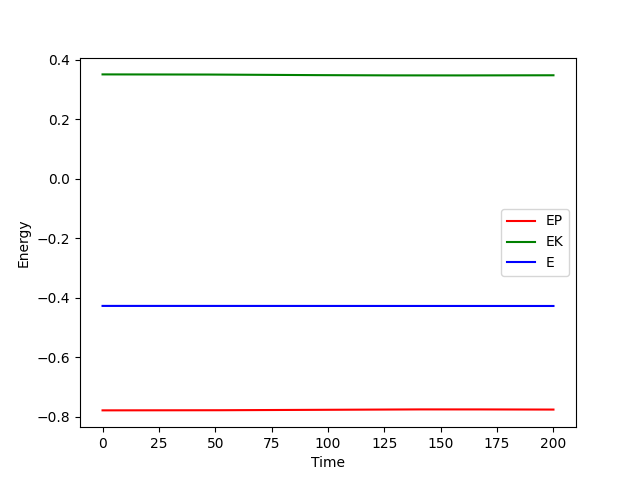
\includegraphics[width=\textwidth]{chapters/results/img/pm-galaxy/energy.png}
        \caption{Energy}
        \label{fig:physical-quantities-pm-sub1}
    \end{subfigure}
    \hfill
    \begin{subfigure}[b]{0.45\textwidth}
        \centering
        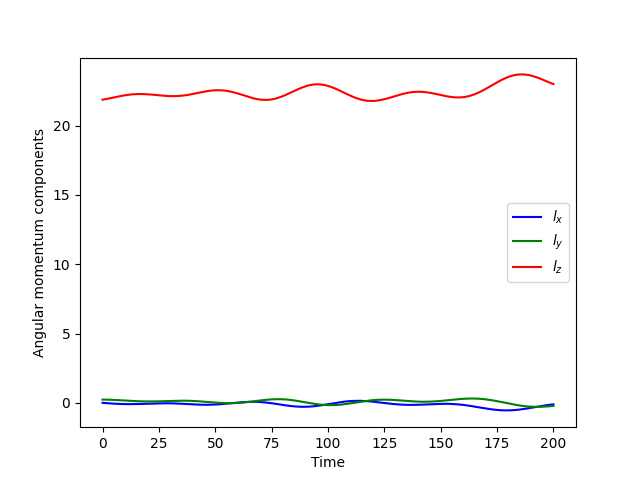
\includegraphics[width=\textwidth]{chapters/results/img/pm-galaxy/angular-momentum.png}
        \caption{Angular momentum}
        \label{fig:physical-quantities-pm-sub2}
    \end{subfigure}

    \vspace{0.2cm}

    \begin{subfigure}[b]{0.45\textwidth}
        \centering
        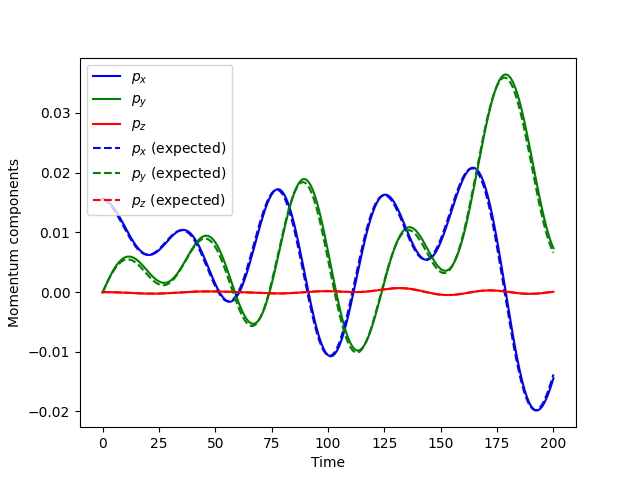
\includegraphics[width=\textwidth]{chapters/results/img/pm-galaxy/momentum.png}
        \caption{Momentum; broken lines represent the expected momentum following \autoref{eq:expected-momentum-change}}
        \label{fig:physical-quantities-pm-sub3}
    \end{subfigure}

    \caption{Fundamental physical quantities describing the system over time in the PM simulation.
        Time is in Myr, and the quantities are expressed in units consistent with \autoref{tab:galaxy-parameters}}
    \label{fig:physical-quantities-pm}
\end{figure}

\subsection{\texorpdfstring{\PThreeM{}}{P3M} method}
The \PThreeM{}-based simulation uses the same parameters as the PM method.
The reference force was calculated using the $S_1$ shape formula (\autoref{eq:s1-reference-force}) with particle diameter $a=3H$.
The cutoff radius was set to $r_e=0.7a$.
One extra free parameter is the \textit{softening length} $\epsilon$, which modifies the universal law of gravitation so that division by zero can be avoided, i.e., the modified law is
\begin{equation*}
    F^\text{soft}_{ij}(r) = \frac{G m_i m_j}{r_{ij}^2 + \epsilon^2}.
\end{equation*}
In the simulation, $\epsilon$ was set arbitrarily to $1.5$ kpc.
The whole configuration of the \PThreeM{} method is conveniently shown in \autoref{tab:p3m-method-parameters}.
The system's evolution is presented in \autoref{fig:spiral-galaxy-evolution-p3m}, and the graphs of energy, angular momentum, and momentum components vs. time are shown in \autoref{fig:physical-quantities-p3m}.

\subsection{Barnes-Hut algorithm}
For the Barnes-Hut algorithm test, the initial conditions of the system remain the same as in the two previous simulations.
The softening length $\epsilon$ was set to 1 kpc, and quadrupole terms were omitted.
The whole configuration of the method is shown in \autoref{tab:bh-method-parameters}.
The snapshots of the simulation are displayed in \autoref{fig:spiral-galaxy-evolution-bh}, and the graphs showing how the energy, momentum, and angular momentum varied over time are shown in \autoref{fig:physical-quantities-bh}.

\subsection{Commentary}
All of the implemented methods successfully reproduced the expected structural features of a spiral galaxy.
A region of high density is clearly localized in the center of the galaxy, and characteristic spiral arms emerge around the 150 Myr mark.
The snapshots from all three simulations (\autoref{fig:spiral-galaxy-evolution-pm}, \autoref{fig:spiral-galaxy-evolution-p3m}, and \autoref{fig:spiral-galaxy-evolution-bh}) show similar evolution of the system over time, with the last snapshot of each simulation visually resembling a real-world spiral galaxy (cf. \autoref{fig:ngc-628}).
It is worth noting, however, that the system evolves more rapidly in the PM-based simulation.
For instance, the spiral arms are significantly more developed at $t = 100$ Myr (\autoref{fig:spiral-galaxy-evolution-pm-sub2}) compared to the same time point in the simulations using the other two methods.
This accelerated evolution is likely due to the smaller ``induced softening length'' inherent to the PM method, which results in stronger gravitational forces. These limitations were anticipated and discussed in \autoref{subsubsec:pm-global-picture}.

Energy plots (\autoref{fig:physical-quantities-pm-sub1}, \autoref{fig:physical-quantities-p3m-sub1}, and \autoref{fig:physical-quantities-bh-sub1}) show that each of the methods tested conserved the total energy.
The plots of angular momentum over time (\autoref{fig:physical-quantities-pm-sub2}, \autoref{fig:physical-quantities-p3m-sub2}, and \autoref{fig:physical-quantities-bh-sub2}) illustrate that the angular momentum was \textit{on average} constant with the variations stemming from the presence of the external halo field.
Finally, the momentum plots (\autoref{fig:physical-quantities-pm-sub3}, \autoref{fig:physical-quantities-p3m-sub3}, and \autoref{fig:physical-quantities-bh-sub3}) demonstrate that the $z$-component of the momentum vector remains constant, while the remaining components change (again due to the external field).
The comparison of the actual values of the momentum with the theoretical values, updated in each timestep according to \autoref{eq:expected-momentum-change}, shows that the change in the $x$- and $y$-components is correct.
